\chapter{State of the art}

\section{Cloud storage services} \label{cloud_storage_services}

Cloud storage services have been steadily increasing in popularity and reached mainstream status in the past decade. In essence, these services allow users to upload and store files on the internet without the need to own the physical storage medium. Files can be accesed from almost any ``smart'' consumer device with an internet connection, provided that the user follows the required authentication process.

Most cloud storage services provide free plans, which usually limit the total storage capacity. Their premium plans either follow the subscription business model or even go as far as to require a one-time purchase in exchange for a lifetime subscription.~\cite{get_3tb_of_lifetime_cloud_storage}

As of \monthyeardate\today, some of the most popular names ring a bell even to non-technical users:
\begin{itemize} \label{lst:cloud_storage_services}
\itemsep0em
\item Microsoft OneDrive -- 115 million customers between \date{2007} and \date{2017}~\cite{10_years_of_onedrive}
\item Google Drive -- 800 million active users, \date{March 2017}~\cite{google_plans_to_leverage,google_updates_drive_focus_on_business}
\item Apple iCloud Drive -- a subsystem of Apple iCloud, which reached 782 million users in \date{February 2016}~\cite{icloud_hits_782m_users}
\item Box Drive -- 47 thousand paying customers as of \date{August 2015}~\cite{box_hires_nasdaq_exec}
\item Dropbox -- 500 million registered users, 10 million paying users as of \date{December 2017}~\cite{dropbox_inc_registration_statement}
\end{itemize}

This is no coincidence. It is a common practice among tech companies to attempt to draw users into their own ecosystem, especially when it is a vast one. Consumers that already use several products owned by the same company tend to favor that company's other products over their direct competitors'. There are multiple advantages in doing so. For one, familiarity is a key factor. A competitor's service may be more difficult to use by a consumer who is unfamiliar with it. In addition, a single ecosystem provides greater cohesion between its different elements. This translates into better integration between services, which improves the overall user experience.

Two of the largest technology companies -- \mbox{Apple Inc.} and \mbox{Alphabet Inc.} -- are commonplace examples of this strategy. Users who sign up for a free Gmail account automatically receive an associated \mbox{15 GB} storage plan on Google Drive. Moreover, this storage is shared among three different services: Google Drive, Gmail and Google Photos. Similarly, Apple offers \mbox{5 GB} of free storage on iCloud:

\begin{quoting}[vskip=0pt]
\emph{iCloud is built into every Apple device. That means all your stuff — photos, files, notes, and more — is safe, up to date, and available wherever you are. And it works automatically, so all you have to do is keep doing what you love. Everyone gets \mbox{5 GB} of free iCloud storage to start, and it’s easy to add more at any time.}~\cite{icloud_website}
\end{quoting}

It seems that offering free storage is similar in concept to planting a seed that will reap a greater harvest. Indeed, making a user familiar with your service will make him more likely choose your premium plan when deciding to upgrade, instead of your competitor's.

\section{User Interface}

All services mentioned in listing \ref{lst:cloud_storage_services} support user interaction through web platforms. These interfaces allow users to manage their files and data from a web browser, which is an ubiquitous piece of software.

These interfaces are updated regularly with new features and improved design. In \date{May 2018}, Google rolled out a new update\cite{google_drive_ui_updates} for Drive which is more in tune with its latest material design principles\cite{how_google_created_a_custom_material_theme}. Some of the changes can be observed in figures~\ref{fig:drive-before} and~\ref{fig:drive-after}.

\begin{figure}[bpt]
\caption{Google Drive before redesign. Source:~\cite{google_drive_ui_updates}}
\label{fig:drive-before}
\centering
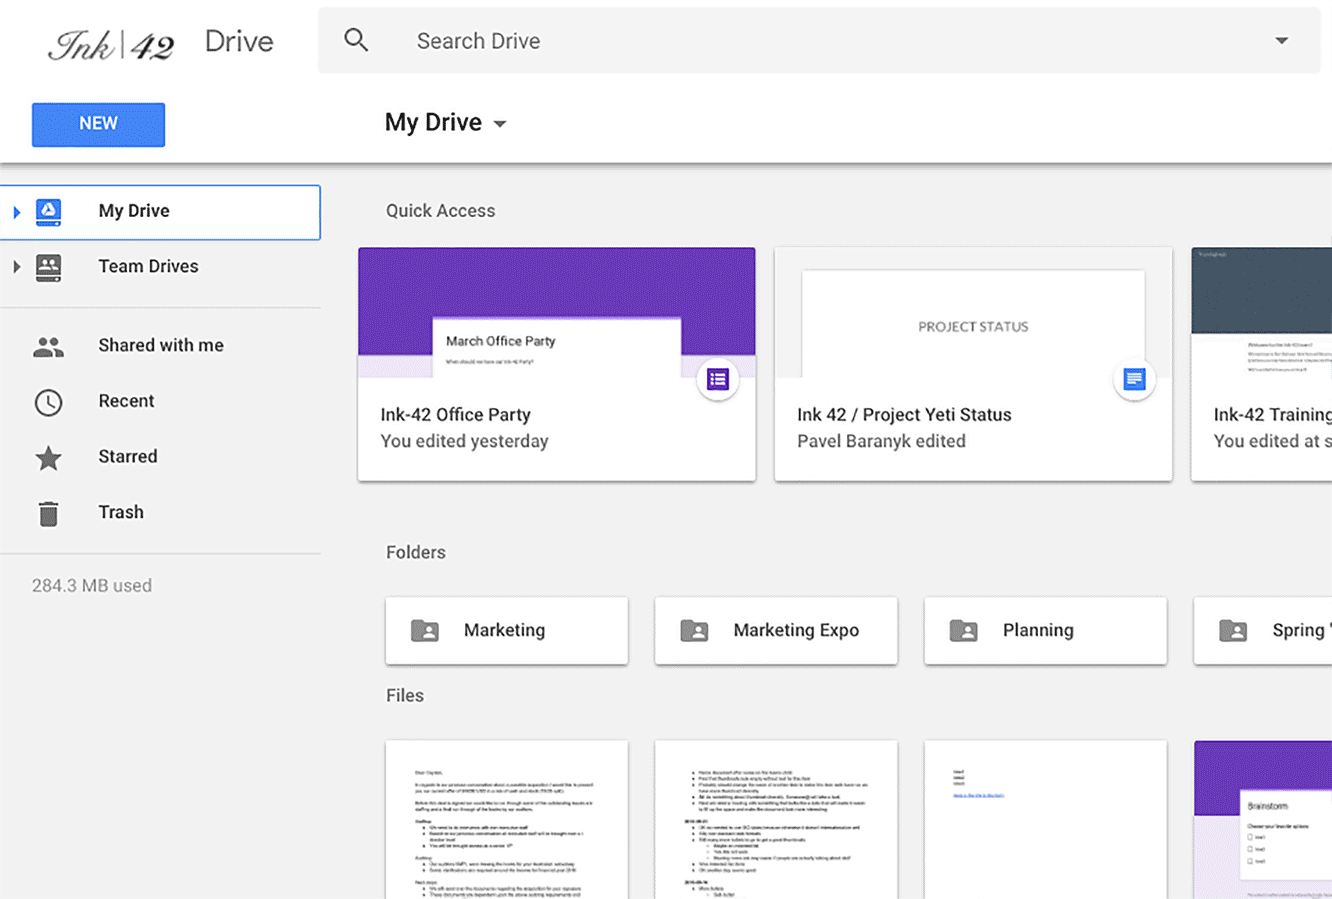
\includegraphics[width=\linewidth]{drive-before}
\end{figure}

\begin{figure}[bpt]
\caption{Google Drive after redesign. Source:~\cite{google_drive_ui_updates}}
\label{fig:drive-after}
\centering
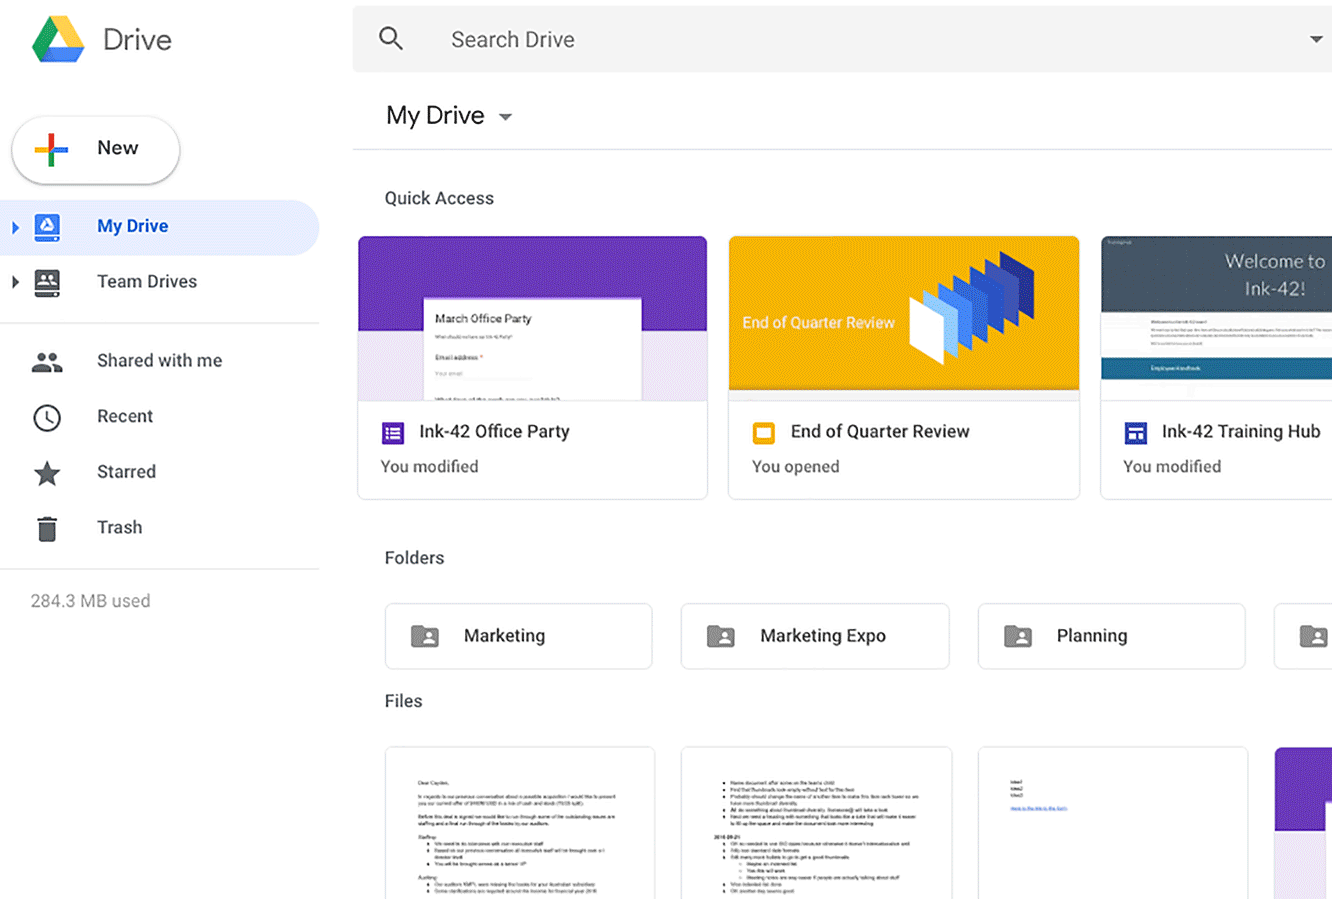
\includegraphics[width=\linewidth]{drive-after}
\end{figure}


A secondary medium is represented by mobile applications. As of \monthyeardate\today, Google Drive for Android has been installed more than one billion times~\cite{google_drive_android_app}. Dropbox and OneDrive are close behind, with more than 500 million and 100 million installs, respectively~\cite{dropbox_android_app,one_drive_android_app}.

\section{File Sync}

Originally, users did not interact with cloud storage services as they do today. When Dropbox was initially founded in 2007, it did not rely on a web interface for its service. It did not even own the \emph{dropbox.com} domain~\cite{dropbox_acquires_dropbox_dot_com}. Users had to download a desktop application from \url{getdropbox.com} and run it locally, thus interacting with the service.

The application followed an approach that was mainly designed by Andrew Houston, the company's CEO. The key element was a special folder added to the user's file system. This folder was then synced to all devices that were linked to the same Dropbox account. Any file placed in this folder would get sent to the cloud and become available to other devices.

The success of Dropbox convinced other companies to follow suit. Google Drive was introduced in \date{April 2012} for Windows, macOS and Android~\cite{introducing_google_drive}. A few months later, an iOS application was launched as well~\cite{hands_on_with_the_google_drive_for_ios_app}.

In the same year, Google famously told users: ``We're working on Linux support -- hang tight!''~\cite{google_drive_for_linux_is_on_the_way}. The announcement went under the radar and the project was eventually cancelled. This gave birth to an infamous joke website which counts how much time users have been waiting for the Linux client~\cite{how_long_since_google_said_hang_tight}.

In \date{September 2017}, Google made another announcement regarding the desktop application. The official Drive app would be discontinued in \date{March 2018}, its place being taken by the new \emph{Backup and Sync} app~\cite{introducing_backup_and_sync,google_drive_is_being_replaced_by_backup_and_sync}.

It is easy to notice then that Linux users have been at a disadvantage ever since Drive was first launched. They essentially had three options: switch to a different storage service or operating system, use the web platform, or use unofficial third-party clients, which were usually bugged and lacked complete functionality.

\section{Main advantages}

\subsection{Cloud Storage}

Many technology consumers and enthusiasts use cloud storage services on a daily basis. Compared to traditional disk-based storage systems, cloud-based services provide several advantages. The most palpable one is data redundancy and backup. Users no longer risk the chance of losing their data due to a lost or stolen device or because of a hardware failure. Files that are stored in the cloud provide an extra layer of safety. On top of this, file sharing becomes almost trivial. What used to require manual transfers between different storage mediums (e.g. floppy disks, CDs, flash drives or external hard drives) is now done almost entirely automatically. It is enough to place the desired files in the special folder on a computer and they will appear on all other linked devices.

Indeed, this is the inconvenience that gave birth to Dropbox. Andrew Houston founded the company after repeatedly forgetting his USB flash drive while being a student at MIT~\cite{how_the_habit_of_forgetting}.

Another advantage is cross-platform integration. Over a third of the world's population owns a smartphone, and this number is expected to grow in the coming years~\cite{smartphone_ownership_usage_and_penetration_by_country}. Therefore, cloud storage services narrow the gap between traditional desktop computers and mobile phones.

Finally, the freemium model adopted by many of the services mentioned previously translates into free extra storage for everyday users. Even the paid plans are a strong competitor for traditional storage systems. In \date{2018}, the cost per gigabyte of storage commonly reaches values as low as \mbox{\textdollar 0.05\slash GB}~\cite{hard_drive_cost_per_gigabyte}. With Google Drive's most popular paid plan, this value is approximately 4 times lower: \mbox{\textdollar 0.012\slash GB\slash month} \cite{google_drive_pricing}. Although this is a recurrent cost, it often makes sense financially to opt for cloud storage, especially with all the other provided benefits.

\subsection{File Sync}

File syncing is in itself an enticing feature. Having a special folder on an existing file system comes with no additional learning curve. Any computer-literate user can instantly make sense of such a service and use it without prior preparation. Having the data physically present on the local storage system makes it readily available and still accessible even in the absence of an internet connection.

\subsection{Service Integration}

As discussed above, file sharing services are seldom provided by themselves. The best example of this is Google, which aims to merge most of its services into a cohesive and consistent user experience. Special files created in Google Docs, Forms, Sheets or Slides use Drive as the storage medium and integrate with it seamlessly. Files can easily be shared with Gmail contacts. Mail attachments can be saved to Drive with a single click. This improves workflow of many consumers globally. Teams no longer have to pass text documents back and forth; all members can edit the same document at the same time.

\section{Main disadvantages}

\subsection{Security}

Although useful in many aspects, the rise of cloud storage services are a cause for worry for many users. One of the main concern comes from the risk associated with storing sensitive information on someone else's servers, making it vulnerable to data breaches and leaks.

Dropbox is just one case of controversy. In \date{June 2011} an authentication problem allowed the access of multiple accounts for several hours \emph{without} passwords.\cite{dropbox_security_bug_made_passwords_optional_for_four_hours} In \date{August 2016}, 68 million accounts have been compromised by hackers who stole email addresses and hashed passwords.\cite{dropbox_hackers_stole_email_addresses}

\subsection{Availability}

Throughout the years, web services in general have proved that 100\% reliability is unachievable in practice. Google offers a 99.9\% uptime guarantee for G Suite customers of Google Drive. However, there have been multiple outages since the service's initial launch in 2012:

\begin{itemize}
  \itemsep0em
  \item \date{March 2013}\cite{google_drive_experiencing_outage}
  \item \date{October 2014}\cite{google_drive_and_docs_down}
  \item \date{January 2016}\cite{gmail_google_drive_down}. Google later apologized:
    \begin{quote}
      At Google we recognize that failures are statistically inevitable, and we strive to insulate our users from the effects of failures. As that did not happen in this instance, we apologize to everyone who was inconvenienced by this event. Our engineers are conducting a post-mortem investigation to determine how to make our services more resilient to unplanned network failures, and we will do our utmost to continue to make Google service outages notable for their rarity.
    \end{quote}
  \item \date{September 2017}\cite{google_suffered_a_meltdown}
\end{itemize}

These outages carry an immense impact on users. When all Google services went out for 5 minutes in \date{August 2013}, the total internet traffic dropped by 40\%.\cite{google_goes_down_for_5_minutes} Even so, Google Drive's reliability still beats that of user-owned hardware. Consumers are more likely to lose data because of their own hard drives failing than Google's. Still, the perceived effect is the opposite. When you lose your data, you might be tempted to pass it off as a fact of life. When Google loses your data, there is outrage, and rightly so.

\subsection{Power user experience} \label{power_user_experience}

Although cloud hosting services usually provide a first-rate user experience, they do not cover every possible use case. This is especially true when discussing about power users. For the purpose of this argument, I will use the following definition of the term:

\fbox{\textit{(noun)} \textbf{power user}: a knowledgeable and sophisticated user of computers.}

This includes students, professional programmers, hobbyists and all other computer users with a large knowledge base who like to tinker with computers in interesting and unexpected ways.

This description matches the traditional stereotype of a computer hacker. The term is known in popular press as someone who breaks into computers. However, it has a different meaning among programmers. In this context, a hacker is usually someone who strikes to achieve mastery by their own merit, being driven by curiosity more often than not. It is not necessarily a computer term: a famous anecdote regarding Nobel laureate Richard Feynman describes his pastime of breaking into safes containing secret documents just for the fun of it\cite{feynman}.

Hackers often create wealth by writing open source software and publishing it for the entire world to use and modify freely\cite{hackers_and_painters}. Plenty of them come into contact with programming at an early age and follow formal education only as a secondary way of learning. Hackers are seldom happy with their systems and their knowledge. They always seek new and better ways of making computers do what they want. Living in the terminal usually becomes the preferred way of getting things done.

For many of them, it is hard to take slow typists seriously as programmers. This is not an indicator of arrogance -- typing speed does not reflect one's ability as a programmer, but it does show much time one has spent using a computer, actually writing programs.

Although Linux has a modest market share of only 2.16\% for desktop and laptop usage\cite{linux_market_share}, it is far more popular with developers and power users, 48.3\% of them having used a variation of it for development work in \date{2018}.\cite{stack_overflow_developer_survey_results}

It is therefore unfortunate that the very people who create software are the ones who benefit the least from it, at least in the case of cloud hosting services. Forcing a power user to use a browser in order to share files can easily be an impediment to their productivity. The command line simply does not pair well with browser-based web services. Imagine wanting to write a script that uploads some backup file to such a service and having to implement it in a way that integrates it into the browser. This sort of automation task is not unheard of among power users, yet the lack of native Linux support makes it way harder than it has to be.
